% Options for packages loaded elsewhere
\PassOptionsToPackage{unicode}{hyperref}
\PassOptionsToPackage{hyphens}{url}
%
\documentclass[
]{book}
\usepackage{lmodern}
\usepackage{amssymb,amsmath}
\usepackage{ifxetex,ifluatex}
\ifnum 0\ifxetex 1\fi\ifluatex 1\fi=0 % if pdftex
  \usepackage[T1]{fontenc}
  \usepackage[utf8]{inputenc}
  \usepackage{textcomp} % provide euro and other symbols
\else % if luatex or xetex
  \usepackage{unicode-math}
  \defaultfontfeatures{Scale=MatchLowercase}
  \defaultfontfeatures[\rmfamily]{Ligatures=TeX,Scale=1}
\fi
% Use upquote if available, for straight quotes in verbatim environments
\IfFileExists{upquote.sty}{\usepackage{upquote}}{}
\IfFileExists{microtype.sty}{% use microtype if available
  \usepackage[]{microtype}
  \UseMicrotypeSet[protrusion]{basicmath} % disable protrusion for tt fonts
}{}
\makeatletter
\@ifundefined{KOMAClassName}{% if non-KOMA class
  \IfFileExists{parskip.sty}{%
    \usepackage{parskip}
  }{% else
    \setlength{\parindent}{0pt}
    \setlength{\parskip}{6pt plus 2pt minus 1pt}}
}{% if KOMA class
  \KOMAoptions{parskip=half}}
\makeatother
\usepackage{xcolor}
\IfFileExists{xurl.sty}{\usepackage{xurl}}{} % add URL line breaks if available
\IfFileExists{bookmark.sty}{\usepackage{bookmark}}{\usepackage{hyperref}}
\hypersetup{
  pdftitle={Roberta Spencer Family \& Friends COOKBOOK},
  pdfauthor={The Spencers},
  hidelinks,
  pdfcreator={LaTeX via pandoc}}
\urlstyle{same} % disable monospaced font for URLs
\usepackage{longtable,booktabs}
% Correct order of tables after \paragraph or \subparagraph
\usepackage{etoolbox}
\makeatletter
\patchcmd\longtable{\par}{\if@noskipsec\mbox{}\fi\par}{}{}
\makeatother
% Allow footnotes in longtable head/foot
\IfFileExists{footnotehyper.sty}{\usepackage{footnotehyper}}{\usepackage{footnote}}
\makesavenoteenv{longtable}
\usepackage{graphicx,grffile}
\makeatletter
\def\maxwidth{\ifdim\Gin@nat@width>\linewidth\linewidth\else\Gin@nat@width\fi}
\def\maxheight{\ifdim\Gin@nat@height>\textheight\textheight\else\Gin@nat@height\fi}
\makeatother
% Scale images if necessary, so that they will not overflow the page
% margins by default, and it is still possible to overwrite the defaults
% using explicit options in \includegraphics[width, height, ...]{}
\setkeys{Gin}{width=\maxwidth,height=\maxheight,keepaspectratio}
% Set default figure placement to htbp
\makeatletter
\def\fps@figure{htbp}
\makeatother
\setlength{\emergencystretch}{3em} % prevent overfull lines
\providecommand{\tightlist}{%
  \setlength{\itemsep}{0pt}\setlength{\parskip}{0pt}}
\setcounter{secnumdepth}{5}
\usepackage{wrapfig}

\title{Roberta Spencer Family \& Friends COOKBOOK}
\author{The Spencers}
\date{2021-03-20}

\begin{document}
\maketitle

{
\setcounter{tocdepth}{1}
\tableofcontents
}
\hypertarget{introduction}{%
\chapter{Introduction}\label{introduction}}

This is the Spencer Family \& Friends Cookbook

dedicated to our mother Roberta Belle Spencer who taught us the joy of:

Cooking

Sharing

Eating

Left-overs

Vivamus vehicula leo a justo. Quisque nec augue. Morbi mauris wisi, aliquet vitae, dignissim eget, sollicitudin molestie, ligula. In dictum enim sit amet risus. Curabitur vitae velit eu diam rhoncus hendrerit. Vivamus ut elit. Praesent mattis ipsum quis turpis. Curabitur rhoncus neque eu dui. Etiam vitae magna. Nam ullamcorper. Praesent interdum bibendum magna. Quisque auctor aliquam dolor. Morbi eu lorem et est porttitor fermentum. Nunc egestas arcu at tortor varius viverra. Fusce eu nulla ut nulla interdum consectetuer. Vestibulum gravida.

\begin{wrapfigure}{R}{0.7\textwidth}

\hfill{}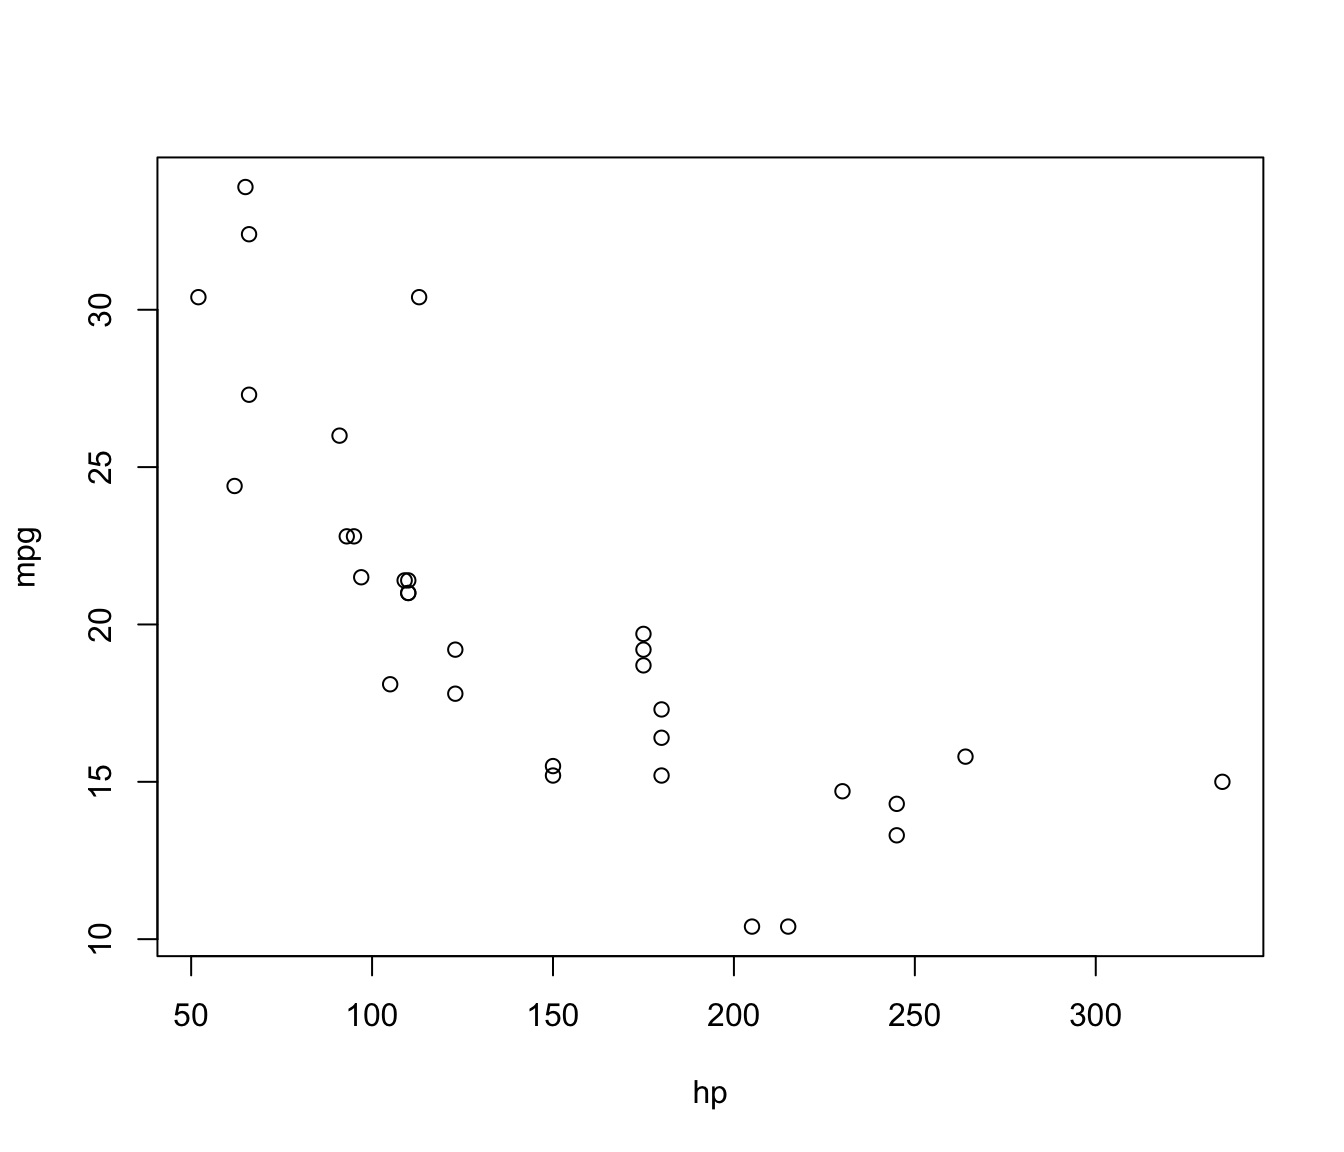
\includegraphics[width=.7\textwidth]{spencerfamilycookbook_files/figure-latex/unnamed-chunk-2-1} 

\caption{My Flowchart}\label{fig:unnamed-chunk-2}
\end{wrapfigure}

Morbi mattis libero sed est. Vivamus vehicula leo a justo. Quisque nec augue. Morbi mauris wisi, aliquet vitae, dignissim eget, sollicitudin molestie, ligula. In dictum enim sit amet risus. Curabitur vitae velit eu diam rhoncus hendrerit. Vivamus ut elit. Praesent mattis ipsum quis turpis. Curabitur rhoncus neque eu dui. Etiam vitae magna. Nam ullamcorper. Praesent interdum bibendum magna. Quisque auctor aliquam dolor. Morbi eu lorem et est porttitor fermentum. Nunc egestas arcu at tortor varius viverra. Fusce eu nulla ut nulla interdum consectetuer. Vestibulum gravida. Morbi mattis libero sed est.

\begin{wrapfigure}{R}{.25\textwidth}  
 \begin{center}
    
\includegraphics[width=.2\textwidth]{"images/500.jpg"}
  \caption{Diamonds} 
\end{center}
\end{wrapfigure}

Morbi mattis libero sed est. Vivamus vehicula leo a justo. Quisque nec augue. Morbi mauris wisi, aliquet vitae, dignissim eget, sollicitudin molestie, ligula. In dictum enim sit amet risus. Curabitur vitae velit eu diam rhoncus hendrerit. Vivamus ut elit. Praesent mattis ipsum quis turpis. Curabitur rhoncus neque eu dui. Etiam vitae magna. Nam ullamcorper. Praesent interdum bibendum magna. Quisque auctor aliquam dolor. Morbi eu lorem et est porttitor fermentum. Nunc egestas arcu at tortor varius viverra. Fusce eu nulla ut nulla interdum consectetuer. Vestibulum gravida. Morbi mattis libero sed est.

Oh yea? Well the same back at you !

\hypertarget{notes}{%
\chapter{NOTES}\label{notes}}

\hypertarget{notes}{%
\section*{What's the Difference Between Chop, Dice, and Mince?}\label{notes}}


\hypertarget{i-dont-know-but-try-these-comments}{%
\subsection*{I don't know but try these comments}\label{i-dont-know-but-try-these-comments}}


Sometimes the words chop and dice are used interchangeably, but technically the word dice is used for smaller pieces and the word chop is used for larger pieces.
You seldom see the term large dice, but you will see large chop and small dice rather frequently. Dice can also refer to cutting vegetable into cubes of a specific size while chop is less precise. In general, chop is more casual and has more leeway while dice is more specific.
The word mince means a very small dice.

\hypertarget{how-big-is-a-dice-how-small-is-a-mince}{%
\subsection*{How Big is a Dice? How Small is a Mince?}\label{how-big-is-a-dice-how-small-is-a-mince}}


How do you know how big or small something is supposed to be? If the recipe writer feels it matters,
usually they will also include a measurement, like 3/4" dice.
Again, we see the word dice here to indicate that this is a very specific direction.
But if the sizing has some leeway, they will say either large, medium or small chop. Unfortunately,
these sizes aren't standardized so it's hard to give measurements.

\begin{itemize}
\item
  Large chop -- For me, when a recipe says large chop, I usually make it roughly the size of a nickel.
\item
\item
  Medium Chop -- Medium chop is about half the size of a nickel.
\item
\item
  Diced (Small Chop) -- Small chop is about half of medium chop, perhaps a quarter inch to a side.
\item
\item
  Minced -- Mince is very fine, as small as I can get it.
\end{itemize}

\hypertarget{appetizers}{%
\chapter{Appetizers and Beverages}\label{appetizers}}

\hypertarget{artichoke-dip}{%
\section*{ARTICHOKE DIP}\label{artichoke-dip}}


\hypertarget{chef-debbie-wescott}{%
\subsection*{Chef: Debbie Wescott}\label{chef-debbie-wescott}}


\hypertarget{ingredients}{%
\subsection*{Ingredients}\label{ingredients}}


\begin{itemize}
\tightlist
\item
  2 8oz packages of cream cheese - softened
\item
  1/2 cup mayonnaise
\item
  3 to 5 cloves of garlic (or 3 tablespoons of Minced garlic)
\item
  14 oz can artichoke hearts drained and chopped - marinated
\item
  10 oz package of frozen spinach - softened
\item
  2 tablespoons of lemon juice
\item
  1/2 cup grated parmesan cheese
\item
  1 cup of mozzoretta cheese - grated
\end{itemize}

\hypertarget{directions}{%
\subsection*{Directions}\label{directions}}


Cream the cream cheese, mayonnaise and garlic together and set aside.
Mix remaining ingredients down the list to Parmesan cheese.
Combine parts 1 and 2 and spread into a baking dish.
Bake at 375 deg for 20 minutes then layer on Mozzoretta cheese,
Bake 5 more minutes until light golden brown.
Serve with fresh veggies or crackers.
YUM!

\begin{center}\rule{0.5\linewidth}{0.5pt}\end{center}

\hypertarget{cowboy-caviar}{%
\section*{COWBOY CAVIAR}\label{cowboy-caviar}}


\hypertarget{chef-patricia-blair}{%
\subsection*{Chef: Patricia Blair}\label{chef-patricia-blair}}


\hypertarget{ingredients-1}{%
\subsection*{Ingredients}\label{ingredients-1}}


\begin{itemize}
\tightlist
\item
  15oz can black eyed peas - drained
\item
  15oz can \href{https://en.wikipedia.org/wiki/Shoepeg_corn}{shoepeg corn} - drained
\item
  2/3 cup cilantro - chopped
\item
  2/3 cup green onion - chopped
\item
  1/4 cup olive oil dressing
\item
  1/4 cup red wine vinegar
\item
  2 cloves garlic - minced
\item
  3/4 teaspoon salt
\item
  1/8 teaspoon pepper
\item
  1/2 teaspoon cumin
\item
  2 large tomatoes - diced
\item
  2 avacados - diced
\end{itemize}

\hypertarget{directions-1}{%
\subsection*{Directions}\label{directions-1}}


Except the tomatoes and avacados marinate all other ingredients together for 6+ hours. Add diced tomatoes and avacados 30 minutes before serving.

\begin{center}\rule{0.5\linewidth}{0.5pt}\end{center}

\hypertarget{cream-of-coconut-fruit-dip}{%
\section*{CREAM OF COCONUT FRUIT DIP}\label{cream-of-coconut-fruit-dip}}


\hypertarget{chef-jennifer-gustin}{%
\subsection*{Chef: Jennifer Gustin}\label{chef-jennifer-gustin}}


\hypertarget{ingredients-2}{%
\subsection*{Ingredients}\label{ingredients-2}}


\begin{itemize}
\tightlist
\item
  1 package instant vanilla pudding (4.6 oz)
\item
  1 container cream of coconut (found in alchol mix section)
\item
  16 oz whipped cream (Cool Whip)
\end{itemize}

\hypertarget{directions-2}{%
\subsection*{Directions}\label{directions-2}}


Combine all three ingredients together and chill for one hour so pudding dissolves completely.
Serve with fruit. Great with sliced apple.

\begin{center}\rule{0.5\linewidth}{0.5pt}\end{center}

\hypertarget{cucumber-sandwiches}{%
\section*{CUCUMBER SANDWICHES}\label{cucumber-sandwiches}}


\hypertarget{chef-patricia-blair-1}{%
\subsection*{Chef: Patricia Blair}\label{chef-patricia-blair-1}}


\hypertarget{ingredients-3}{%
\subsection*{Ingredients}\label{ingredients-3}}


\begin{itemize}
\tightlist
\item
  8 oz cream cheese
\item
  2 tablespoons mayonnaise
\item
  2 green onions - diced
\item
  1/2 teaspoon \href{https://www.mccormick.com/gourmet/recipes/other/bon-appetit-seasoning-replacement}{Bon Appettit} seasoning
\item
  1/2 teaspoon dill weed
\item
  1/2 teaspoon garlic salt
\item
  cucumbers - peeled and sliced
\item
  tomatoes - sliced
\item
  bread - crust removed
\end{itemize}

\hypertarget{directions-3}{%
\subsection*{Directions}\label{directions-3}}


Combine together: cream cheese, mayonnaise, green onions, Bon Appettit, dill weed, and garlic salt.
Spread mixture on bread and layer with sliced cucumber and tomato. Cover and refrigerate until ready to use.

\begin{center}\rule{0.5\linewidth}{0.5pt}\end{center}

\hypertarget{dads-sunday-evening-popcorn}{%
\section*{DAD'S SUNDAY EVENING POPCORN}\label{dads-sunday-evening-popcorn}}


\hypertarget{chef-alvin-spencer}{%
\subsection*{Chef: Alvin Spencer}\label{chef-alvin-spencer}}


\hypertarget{ingredients-4}{%
\subsection*{Ingredients}\label{ingredients-4}}


\begin{itemize}
\tightlist
\item
  1/2 cup of popcorn - uncooked
\item
  1 to 3 teaspoons of olive oil
\item
  1/4 cup of butter or margerine
\item
  1/4 teaspoon of popcorn salt
\end{itemize}

\hypertarget{directions-4}{%
\subsection*{Directions}\label{directions-4}}


Best cooked in a \href{https://www.whirleypopshop.com/}{Whirley-pop} popcorn popper. This requires only 1 teaspoon of oil.\\
Cook over medium high heat until kernels stop popping or until smoke fills the kitchen.
Place in a large bowel and sprinkle melted butter lightly over popcorn while stirring. Olive oil can be substituted for margarine.
Sprinkle salt over popcorn and stir. Eat while warm and while watching a good movie with the family gathered around you.

\begin{center}\rule{0.5\linewidth}{0.5pt}\end{center}

\hypertarget{five-layer-avocado-dip}{%
\section*{FIVE LAYER AVOCADO DIP}\label{five-layer-avocado-dip}}


\hypertarget{chef-patricia-blair-2}{%
\subsection*{Chef: Patricia Blair}\label{chef-patricia-blair-2}}


\hypertarget{ingredients-5}{%
\subsection*{Ingredients}\label{ingredients-5}}


\begin{itemize}
\tightlist
\item
  1 can refried beans
\item
  1 can chip bean dip
\item
  2 large avocados - mashed
\item
  1 small can green chilies - diced
\item
  1/2 pint sour cream
\item
  1/4 jar favorite salsa
\item
  garlic / onion salt and pepper
\item
  1/2 cup green onions - chopped
\item
  1 can sliced black olives
\item
  1 lb. favorite shredded cheese
\end{itemize}

\hypertarget{directions-5}{%
\subsection*{Directions}\label{directions-5}}


Layer in 9x13 pan.
-- First Layer: 1 can refried beans and 1 can chip bean dip.
-- Second Layer (Mix together) avocados, green chilies, sour cream, salsa, seasonings.
-- Third Layer: Green onions,
-- Fourth Layer: sliced olives.
-- Fifth Layer: cheese.

Serve with chips

\begin{center}\rule{0.5\linewidth}{0.5pt}\end{center}

\hypertarget{hot-buttered-rum-drink}{%
\section*{HOT BUTTERED `RUM' DRINK}\label{hot-buttered-rum-drink}}


\hypertarget{chef-jennifer-gustin-1}{%
\subsection*{Chef: Jennifer Gustin}\label{chef-jennifer-gustin-1}}


\hypertarget{ingredients-6}{%
\subsection*{Ingredients}\label{ingredients-6}}


\begin{itemize}
\tightlist
\item
  1 1/2 cups brown sugar
\item
  1 3/4 cups powdered sugar
\item
  2 pints vanilla ice-cream
\item
  1/2 teaspoon nutmeg
\item
  1 teaspoon cinnamon
\end{itemize}

\hypertarget{directions-6}{%
\subsection*{Directions}\label{directions-6}}


Soften ice-cream 30 minutes in refrigerator. Mix dry ingredients together.
Cream together dry ingredients with softened ice-cream.
Store in freezer. To serve, use 1 1/2 tsp of batter to a cup of hot water or milk. Add more to taste.

\begin{center}\rule{0.5\linewidth}{0.5pt}\end{center}

\hypertarget{hot-chocolate-mix}{%
\section*{HOT CHOCOLATE MIX}\label{hot-chocolate-mix}}


\hypertarget{chef-roberta-spencer}{%
\subsection*{Chef: Roberta Spencer}\label{chef-roberta-spencer}}


\hypertarget{ingredients-7}{%
\subsection*{Ingredients}\label{ingredients-7}}


\begin{itemize}
\tightlist
\item
  1 25.6 oz package of instant nonfat dry milk (10 2/3 cups)
\item
  1 6 oz jar powdered non-dairy creamer
\item
  2 cups powdered sugar
\item
  1 16 oz can instant chocolate drink mix
\end{itemize}

\hypertarget{directions-7}{%
\subsection*{Directions}\label{directions-7}}


Combine all ingredients, Mix well. Put in a large air tight container.
Label. Store in cool, dry place. Use within 6 months. Makes about 17 cups of hot chocolate mix.

-- For hot chocolate -- add 3 tablespoons of mix to 1 cup hot water.

\begin{center}\rule{0.5\linewidth}{0.5pt}\end{center}

\hypertarget{jalapeno-popper-dip}{%
\section*{JALAPENO POPPER DIP}\label{jalapeno-popper-dip}}


\hypertarget{chef-jennifer-gustin-2}{%
\subsection*{Chef: Jennifer Gustin}\label{chef-jennifer-gustin-2}}


\hypertarget{ingredients-8}{%
\subsection*{Ingredients}\label{ingredients-8}}


\begin{itemize}
\tightlist
\item
  2 packages light cream cheese
\item
  1 cup mahyonnaise
\item
  4 oz chopped green chillies
\item
  3 finely chopped jalepenos (teh more seeds you use the spicier it is)
\item
  1 cup parmesan cheese
\item
  1 cup \href{https://en.wikipedia.org/wiki/Bread_crumbs\#Panko}{panko bread crumbs}
\end{itemize}

\hypertarget{directions-8}{%
\subsection*{Directions}\label{directions-8}}


Stir together cream cheese and mayonnaise until smooth. Stir in green chilies and jalapenos. Pour mixture into oven-safe dish (8X8 works well) and sprinkle with parmesan cheese and bread crumbs.

\begin{center}\rule{0.5\linewidth}{0.5pt}\end{center}

\hypertarget{orange-julius-drink}{%
\section*{ORANGE JULIUS DRINK}\label{orange-julius-drink}}


\hypertarget{chef-lori-hilton}{%
\subsection*{Chef: Lori Hilton}\label{chef-lori-hilton}}


\hypertarget{ingredients-9}{%
\subsection*{Ingredients}\label{ingredients-9}}


\begin{itemize}
\tightlist
\item
  1/2 cup concentrated orange juice
\item
  3/4 cup milk
\item
  1 egg
\item
  1/2 teaspoon vanilla
\item
  1/4 cup sugar
\item
  1 1/2 cups ice
\end{itemize}

\hypertarget{directions-9}{%
\subsection*{Directions}\label{directions-9}}


Put all ingredients in a blender and blend until ice is broken up smooth.
Alter amount of ice to change consistency of the drink.

\begin{center}\rule{0.5\linewidth}{0.5pt}\end{center}

\hypertarget{tortillla-appetizer}{%
\section*{TORTILLLA APPETIZER}\label{tortillla-appetizer}}


\hypertarget{chef-patricia-blair-3}{%
\subsection*{Chef: Patricia Blair}\label{chef-patricia-blair-3}}


\hypertarget{ingredients-10}{%
\subsection*{Ingredients}\label{ingredients-10}}


\begin{itemize}
\tightlist
\item
  8 oz cream cheese
\item
  3 green onions - diced
\item
  4 oz can diced green chilies
\item
  1 teaspoon garlic salt
\item
  Olives - cut (desired amount)
\item
  Cheddar cheese - shreaded (desired amount)
\item
  Flour tortillas
\item
  Toothpicks
\end{itemize}

\hypertarget{directions-10}{%
\subsection*{Directions}\label{directions-10}}


Combine all ingredients. Spread mixture on tortillas. Roll tortilla up and slice into desired thickness.
hold together with a toothpick.

\begin{center}\rule{0.5\linewidth}{0.5pt}\end{center}

\hypertarget{warm-creamy-bacon-dip}{%
\section*{WARM CREAMY BACON DIP}\label{warm-creamy-bacon-dip}}


\hypertarget{chef-debbie-wescott-1}{%
\subsection*{Chef: Debbie Wescott}\label{chef-debbie-wescott-1}}


\hypertarget{ingredients-11}{%
\subsection*{Ingredients}\label{ingredients-11}}


\begin{itemize}
\tightlist
\item
  1 16 oz sour cream
\item
  1 3 oz bacon bits (or make your own)
\item
  2 cups grated cheddar or cheddar jack cheese
\item
  1 cup diced green onions
\end{itemize}

\hypertarget{directions-11}{%
\subsection*{Directions}\label{directions-11}}


Heat oven to 400 deg. Combine all ingredients.
Spread in a 1 quart baking dish. Heat 25 -- 30 minutes until hot.
Serve with veggies or crackers.
Great served in a bread bowl. Easy to double recipe!

\begin{center}\rule{0.5\linewidth}{0.5pt}\end{center}

\hypertarget{wedding-punch}{%
\section*{WEDDING PUNCH}\label{wedding-punch}}


\hypertarget{chef-patricia-blair-4}{%
\subsection*{Chef: Patricia Blair}\label{chef-patricia-blair-4}}


\hypertarget{ingredients-12}{%
\subsection*{Ingredients}\label{ingredients-12}}


\begin{itemize}
\tightlist
\item
  1 can frozen orange juice - large
\item
  1 can frozen lemonade - large
\item
  1 cup of sugar
\item
  1 teaspoon vanilla extract
\item
  1 gallon water
\item
  1 2 liter bottle 7-up
\end{itemize}

\hypertarget{directions-12}{%
\subsection*{Directions}\label{directions-12}}


Mix all the ingredients EXCEPT the 7-up. Freeze in freezer bags.

-- To serve -- soften slightly, put in punch bowl, add the bottle of 7-up.

\hypertarget{salad}{%
\chapter{Soups and Salads \{\#soup\}}\label{salad}}

\hypertarget{black-bean-soup}{%
\section*{BLACK BEAN SOUP}\label{black-bean-soup}}


\hypertarget{chef-patricia-blair-5}{%
\subsection*{Chef: Patricia Blair}\label{chef-patricia-blair-5}}


\hypertarget{ingredients-13}{%
\subsection*{Ingredients}\label{ingredients-13}}


\begin{itemize}
\tightlist
\item
  2 16oz cans black beans - undrained
\item
  1 cup reduced sodium chicken broth
\item
  1 small onion - chopped
\item
  1 teaspoon garlic - minced
\item
  1 16oz jar salsa - thick and chuncky
\item
  4 teaspoons lime juice
\item
  2 teaspoons ground cumin
\item
  1/4 teaspoon crushed red pepper (optional)
\item
  1/3 cup plain yogurt (optional)
\item
  fresh cilantro leaves - chopped (optional)
\item
  nonstick cooking spray
\end{itemize}

\hypertarget{directions-13}{%
\subsection*{Directions}\label{directions-13}}


Place 1 can of beans with liquid and chicken broth in blender or food processor, cover, blend until smooth.
Coat large saucepan with cooking spray, heat over medium -- high heat. Add onion and garlic: cook for 4 to 5 minutes or until onion is tender.
Add blended bean mixture, remaining beans and liquid, salsa, lime juice, cumin, and crushed red pepper.
Bring to boil. Reduce heat to low and cover. Cook, stirring occasionally for 25 to 30 minutes. Serve topped with yogurt, garnish with cilantro.

\hypertarget{brocoli-salad}{%
\section*{BROCOLI SALAD}\label{brocoli-salad}}


\hypertarget{chef-jennifer-gustin-3}{%
\subsection*{Chef: Jennifer Gustin}\label{chef-jennifer-gustin-3}}


\hypertarget{ingredients-14}{%
\subsection*{Ingredients}\label{ingredients-14}}


\begin{itemize}
\tightlist
\item
  2 bunches broccoli
\item
  1/2/ red onion - chopped
\item
  1/4 lb bacon
\item
  3 oz sunflower seeds
\item
  1/2 cup raisins
\item
  1 cup light mayonnaise
\item
  1/2 cup sugar
\item
  2 tablespoons white vinegar
\end{itemize}

\hypertarget{directions-14}{%
\subsection*{Directions}\label{directions-14}}


Cut broccoli into bite size pieces, Chop onion, Cook Bacon and crumble. Combine Broccoli, onion, bacon, and raisons in bowel.
In separate bowl, mix mayonnaise, sugar, and vinegar. Toss with salad. Marinate in refrigerator for one hour.
Mix in sunflower seeds before serving.

\hypertarget{brocoli-cheese-and-potato-soup}{%
\section*{BROCOLI, CHEESE AND POTATO SOUP}\label{brocoli-cheese-and-potato-soup}}


\hypertarget{chef-roberta-spencer-1}{%
\subsection*{Chef: Roberta Spencer}\label{chef-roberta-spencer-1}}


\hypertarget{ingredients-15}{%
\subsection*{Ingredients}\label{ingredients-15}}


\begin{itemize}
\tightlist
\item
  4 medium potatoes - eeled and diced
\item
  4 carrots - peeled and sliced
\item
  1 stalk celery - diced
\item
  6 chicken bullion cubes
\item
  6 cups water
\item
  3 stalks broccoli - cut in bite-sized pieces
\item
  1 qart half/half or milk
\item
  1 to 1 1/2 cups flour
\item
  1/2 cup butter or margarine
\item
  1 to 2 cups cheddar cheese grated
\end{itemize}

\hypertarget{directions-15}{%
\subsection*{Directions}\label{directions-15}}


In a large soup pan add potatoes, carrots, onions, celery, water and bouillon cubes.
Bring to a boil, then simmer until vegetables are tender. Add the broccoli and simmer until tender.

White Sauce:

In another pan add milk and melted butter. Add the flour, beat with wire whisk.
Stir until it becomes thick. (Should be thick like paste). Add to vegetables.
Stir until mixed well with vegetables.
Add desired amount of cheese. If too thick add more milk.

\hypertarget{literature}{%
\chapter{Literature}\label{literature}}

Here is a review of existing methods.

\hypertarget{methods}{%
\chapter{Methods}\label{methods}}

We describe our methods in this chapter.

\hypertarget{applications}{%
\chapter{Applications}\label{applications}}

Some \emph{significant} applications are demonstrated in this chapter.

\hypertarget{example-one}{%
\section{Example one}\label{example-one}}

\hypertarget{example-two}{%
\section{Example two}\label{example-two}}

\hypertarget{final-words}{%
\chapter{Final Words}\label{final-words}}

We have finished a nice book. What do you think?


\includegraphics{images/500.jpg}

\end{document}
